\documentclass[12pt]{book}

\usepackage{cite} 
\usepackage{mathpazo}
\usepackage{booktabs}
\usepackage{bbm}
\usepackage{tikz-cd,mathtools}
\usepackage{tikz}
\usepackage{mathtools}
\usepackage{array}
\usepackage[utf8]{inputenc}
\usepackage[T1]{fontenc}
\usepackage{textcomp}
\usepackage[english]{babel}
\usepackage{amsmath, amssymb}
\usepackage[mathscr]{euscript}
\usepackage{subcaption}
\usepackage[margin=1in]{geometry}
\usepackage{graphicx}
\usepackage{listings}
\usepackage{xcolor}
\graphicspath{ {/home/slaing/ML/thesis/thesis_notepad/images/} }
\newtheorem{theorem}{Theorem}[section]
\newtheorem{lemma}[theorem]{Lemma}
\newtheorem{proposition}[theorem]{Proposition}
\newtheorem{corollary}[theorem]{Corollary}

\usepackage{comment}
\usepackage{hyperref}
\hypersetup{
colorlinks=true,
        linkcolor=blue,
        filecolor=magenta,
        urlcolor=cyan,
}
\urlstyle{same}

\newcommand{\A}{\mathbb{A}}
\newcommand{\N}{\mathbb{N}}
\newcommand{\Z}{\mathbb{Z}}
\newcommand{\Q}{\mathbb{Q}}
\newcommand{\R}{\mathbb{R}}
\newcommand{\C}{\mathbb{C}}
\newcommand{\f}{\mathfrak{f}}
\newcommand{\F}{\mathbb{F}}
\newcommand{\g}{\mathfrak{g}}
\newcommand{\K}{\mathbb{K}}
\renewcommand{\l}{\mathfrak{l}}
\newcommand{\p}{\mathfrak{p}}
\renewcommand{\P}{\mathfrak{P}}
\newcommand{\PP}{\mathbb{P}}
\newcommand{\E}{\mathbb{E}}
\newcommand{\todo}[1]{{\color{red}\bf{TODO: #1}}}


\newenvironment{proof}[1][Proof]{\begin{trivlist}
\item[\hskip \labelsep {\bfseries #1}]}{\end{trivlist}}
\newenvironment{definition}[1][Definition]{\begin{trivlist}
\item[\hskip \labelsep {\bfseries #1}]}{\end{trivlist}}
\newenvironment{example}[1][Example]{\begin{trivlist}
\item[\hskip \labelsep {\bfseries #1}]}{\end{trivlist}}
\newenvironment{remark}[1][Remark]{\begin{trivlist}
\item[\hskip \labelsep {\bfseries #1}]}{\end{trivlist}}

\newcommand{\qed}{\nobreak \ifvmode \relax \else
      \ifdim\lastskip<1.5em \hskip-\lastskip
      \hskip1.5em plus0em minus0.5em \fi \nobreak
      \vrule height0.75em width0.5em depth0.25em\fi}

% figure support
\usepackage{import}
\usepackage{xifthen}
\pdfminorversion=7
\usepackage{pdfpages}
\usepackage{transparent}
\newcommand{\incfig}[1]{%
\def\svgwidth{\columnwidth}
\import{./figures/}{#1.pdf_tex}
}


\pdfsuppresswarningpagegroup=1

\begin{document}
\title{Thesis Notepad of Ideas and Progress etc}
\maketitle
\tableofcontents
\begin{comment}
\chapter{Math formulation of ideas}
\section{Adam Ideas}
The Adam algorithm is applied in the following way. \\
For each iteration $t\in\N$, let $g^{t} := \nabla_{w}L(w)$. The update step is given by 

\begin{align*}
	m^{t+1} &= \beta_1 m^{t} + (1-\beta_1)g^{t} \\
	v^{t+1} &= \beta_2 v^{t} + (1-\beta_2) g^{t} \odot g^{t}\\
	\hat{m}^{t+1} &= \frac{1}{1-\beta_1^{t+1}} m^{t+1} \quad , \quad \hat{v}^{t+1} = \frac{1}{1-\beta_2^{t+1}} v^{t+1}\\
	w^{t+1} &= w^{t} - \eta \frac{\hat{m}^{t+1}}{\sqrt{\hat{v}^{t+1}} +\varepsilon }
\end{align*}

\subsection*{LR scheduler ideas}
It is sometimes the case that a learning rate scheduler $(\eta_{j})_{j\in\N} $ is used in conjunction with Adam. One could also encode a decreasing (resp. increasing) step size by changing the $\varepsilon $ parameter with time. 
\\
Namely, one has update steps of the form 
\[
w^{t+1} = w^{t} - \eta \frac{\hat{m}^{t+1}}{\sqrt{\hat{v}^{t+1}} + \varepsilon_t} \quad \text{instead of} \quad w^{t+1} = w^{t} - \eta_t \frac{\hat{m}^{t+1}}{\sqrt{\hat{v}^{t+1}} +\varepsilon }
\] 
\subsubsection*{probably stupid}
Easiest way to alter the existing adam method in torch is just to find the equivalent learning rate schedule which corresponds to a given  $\varepsilon $ schedule. \\ 	
More explicitely, given some sequence $(\varepsilon _{t})_{t\ge_0} $ and $\eta >0$, what sequence $(\eta_{t})_{t\ge_0 } $ is such that 
\[
w^{t+1} = w^{t} - \eta \frac{\hat{m}^{t+1}}{\sqrt{\hat{v}^{t+1}} + \varepsilon_t} \quad \text{is equialent to} \quad w^{t+1} = w^{t} - \eta_t \frac{\hat{m}^{t+1}}{\sqrt{\hat{v}^{t+1}} +\varepsilon_0 }
\] 
Solving would give:
\[
\eta_t = \frac{(\eta - \eta_t)\sqrt{\text{EMA}_{\beta_2}(g_t^2)} + \eta \varepsilon_0   }{\varepsilon _t}
\]
Ok definitely stupid: can't know lr ahead of time. 
Will just implement directly in torch.
\section*{to also consider}
\begin{itemize}
\item The Frederic Kunstner paper discusses Zipf's law and looking at loss of less common tokens. Shows adam learns the less frequent tokens better than SGD even with no batches
\item the Bernstein paper shows how (without first moment ema) most optimizers (e.g Adam, SGD, Prodigy ) are simply steepest descent wrt to some norm and how different parameters should have different operator norms applied depending on shape and action. Adam chooses infinity norm and kind of so does SignSGD
\item the paper from 2020 "geometry of sign GD" shows that maybe sign methods can sometimes be better. In particular when Hessian is centred near diagonal and when the max eigenvalues are much bigger than average eigenvalues. Also SGD and Adam have some similaraties and are equivalent as params in adam $\to 0$.  Also $\ell_{\infty}$ smoothness is weaker than seperable smoothness and is a  sufficient assumption. 
\item Maybe some discussion on Music Foundation models?  
\item implementation pytorch-optimizer forked repo. Good idea? 
\end{itemize}



\section*{Week of 25th November}
\begin{itemize}
\item Read the Optimization for deep learning: Theory and algorithms document
\item implemented the $\varepsilon $-scheduler to optimizer (\href{https://github.com/sam-laing/torch_optimizer_prototypes}{torch optimizer prototypes} forked from online repo)
\item read the confidential paper sent via slack. 
\item read Dynamics of SGD with Stochastic Polyak Stepsizes:
Truly Adaptive Variants and Convergence
to Exact Solution
\item Began benchmarking Adam variants on some toy datasets in collab: the cluster contract still awaits!

\item Looked at Nikkolo's \href{https://github.com/Niccolo-Ajroldi/plainLM/tree/main}{PlainLM repo} repo
\item tried reading up a bit on best practices of hyperparameter sweeps etc. Some basic questions 
\end{itemize}
\section*{Week of 2 December}
\begin{itemize}
\item Read A Survey on Efficient Training of Transformers
	\begin{itemize}
	\item one proposition is SOAP without accumulation for efficiency
	\item AdaDiag basically uses an SVD of the gradient to precondition the step size which still doing ADAM type things. Might be an interesting thing to try and nest with the NestedMA optimizer.
	\end{itemize}
\item IMPROVING ADAPTIVE MOMENT OPTIMIZATION
VIA PRECONDITIONER DIAGONALIZATION
\item investigating the modula package (\href{https://github.com/modula-systems/modula}{Scalable Optimization in the Modular Norm})
\item Looked over the AdamMini paper
\item looked over Why transformers need Adam: A Hessian Perspective
\end{itemize}

\subsection*{some thoughts}
\begin{itemize}
\item would be interesting to investigate bias correction vs taking some steps with SGD and then initializating adaptive optimizer from there
\item would like to try the bernstein norm and explictely assign a different optimizer paradigm depending on the type of layer as discussed in the paper "Scalable Optimization in the Modular Norm". 
\item What are some reasonable ways for the epsilon scheduler to update. Intuitively a milestones $=$ [] seems useful but maybe a functional relationship could be better? 
generally $\varepsilon $ should increase to have something of a similar affect to the learning rate shrinking but to which extent? is there some theory to be built? 
\item evalute on vision transformers and small language models, RNNs, GNNs etc. to start to see if adaptive optimizers are more a data or model choice or both...
\item Adam usually updates the moving averages per batch but it might be interesting to update more strongly for recent batches since if we use mini batching very quickly we lose info within a single epoch even though it might be nice to retain it
\end{itemize}
\section*{Week of 9 December}
\begin{itemize}
\item The Impact of the Mini-batch Size on the Variance of Gradients in Stochastic Gradient Descent
\item Which Algorithmic Choices Matter at Which Batch
\item Why Do We Need Weight Decayin Modern Deep Learning?
\item AdAdaGrad: Adaptive Batch Size Schemes for Adaptive Gradient Methods
\item Adam mini
\item this muon thing
\end{itemize}



\subsection*{ideas}
\begin{itemize}
\item Work with some adaptive batch size; in the paper AdaBatch: Adaptive Batch Sizes for Training Deep Neural Networks, they implement for vision models. They also call it "adaptive" but really just make a batch size schedule and then make sure the ratio of the learning rate to the batch size remains constant. Also not clear whether they look at the adaptive adam step size or just the fixed learning rate (get the impression it's the latter). Don't see many other papers on this topic and the takeaway of the paper was that performace is similar but since the batch size increases, the later epochs are quicker and therefore training time is reduced.
\item This backPACK package let's us compute the variance of batches (or could just do as in The Impact of the Mini-batch Size on the
Variance of Gradients in Stochastic Gradient Descent). Idea to monitor variance as proxy for batch update size\\
At iteration $t$:\\
Obtain $g_t$ and  $Var g_t$\\
Define controller which takes in the batch size, learning rate, epoch and gradient and controls how large the variance is.

Techniques like Inner Product test, 
\item Which Algorithmic Choices Matter at Which Batch
Sizes? Insights From a Noisy Quadratic Model
\item get partial hessian of some of the diagonal blocks  (the hessian perspective on adam paper shows the structure is basically block diagonal in later epochs). Block diagonal hessian free method kind of ignores the curvature entirely 
\item other network architectures 
\end{itemize}

\section{January 2025}
\subsection*{idea}
Let's consider a harmonic mean of the step size in SGD and the step size in Adam. Note that up to rescaling, the 2 in the harmonic mean formula can be eliminated. 
\begin{align*}
\text{statistic} = \cfrac{1}{\frac{1}{(\frac{\text{EMA}_{\beta_1}(g_k)}{\sqrt{\text{EMA}_{\beta_2}(g_k} }) + \frac{1}{\eta_k}}} = \frac{1}{\frac{\sqrt{\text{EMA}_{\beta_2}}(g_k) }{\text{EMA}_{\beta_1}(g_k)} + \frac{1}{\eta_k}}
\end{align*}
The $\cfrac{1}{\eta_k}$ can be seen as an $\varepsilon_k $ parameter in some sense.\\
However this doesn't seem to extract precisely what we want which is for adam to exactly fall out with an $\varepsilon _k \iff \frac{1}{\eta_k}$ correspondence. It therefore makes sense to maybe search for a step size $s(\beta_1, \beta_2, k)$ for which 
\[
\frac{1}{\frac{1}{s} + \frac{1}{\eta_k}} = \text{Adam step}
\] 
\subsection*{idea}
Investigate the failing of using statistics other than the mean in backpropagation. 
BackPACK provides access to variance for basic networks. However it never seems as though having access to variance actually assists us in making better step sizes. Have begun to design an experiment in which we get the variance of the gradients and the mean each epoch and then compare this to the EMA seen in Adam. Claim that the $v_t^2$ is simply modelling the 2nd moment even though it moving average of exponenets of a sample mean. 
\\
More explicitely, if denote $G_t = \left[ g_{t,1}, \ldots, g_{t, B}  \right] $ so that $g_t = \text{mean}(G_t, \text{dim} = 1) $ for each $t$, we have 
\begin{align*}
v_t^2 = \text{EMA}_{\beta_2}(g_t^2) = \text{EMA}_{\beta_2}\left(\left(  \frac{1}{B}\sum_{b=1}^{B} {g_{t,b}}\right)^2\right) = \text{EMA}_{\beta_2}\left( \frac{1}{B^2} \sum_{b,c}^{} {g_{t,b}g_{t,c}}  \right) 
\end{align*}
It would be interesting to see if as $t\to \infty$, does the distribution parametrized by $m_t$ and  $v_t$ approach the same distirubtion as parametrized by the variance and mean at epoch $t$.
\\
Idea to compute the KL divergence of normals between $(g_t, \text{diag}(\text{Variance}))$ and $(m_t, \text{diag}(v_t - m_t^2)$ and see whether the divergence remains the same, approaches zero, or something else. 
\\
Closed form for two KL divergences is 
\[
D_{KL}(p \,\|\, q) = \frac{1}{2} \left[ \mathrm{tr}(\Sigma_q^{-1} \Sigma_p) + (\mu_q - \mu_p)^\top \Sigma_q^{-1} (\mu_q - \mu_p) - k + \ln\left(\frac{\det\Sigma_q}{\det\Sigma_p}\right) \right]
\] 
made particularly simple where the covariance matrices are diagonal. 
\subsection*{idea}
Understand the distribution of gradients for Adam by plotting the mean and deviation for various dimensions as the iteration grows
\\
maybe understanding just particular blocks is sufficient

\subsection*{idea}
Investigate how signSGD with very large batch sizes works in this paradigm since intuitively the variance should be very low in the case of large batches. 

\subsection*{plainLM}
Forked Niccolo's plainLM repo (\href{https://github.com/sam-laing/minimalLM/tree/main}{minimalLM})
\\
Having some issues and talking to Niccolo tomorrow but will soon be able to run experiments. Namely have the Nested moving average adam variant with an epsilon scheduler. 

\subsection*{more papers}
\begin{itemize}
	\item \href{https://www.andriushchenko.me/assets/pdf/Why Do We Need Weight Decay in Modern Deep Learning.pdf}{weight decay talk from lousanne }
	\item \href{https://arxiv.org/pdf/2310.04415}{D'Angelo et al paper}. Interesting Bias-Variance tradeoff relation. Not really functioning as a true regularizer but changing training dynamics.
	\item \href{https://proceedings.neurips.cc/paper_files/paper/2023/file/040d3b6af368bf71f952c18da5713b48-Paper-Conference.pdf}{gradient norm perspective on weight decay}. Interesting but not really talking about language models. 
	\item after reading Hennig paper connecting signSGD and Adam, looked through some more sign sgd papers but nothing too interesting.
\end{itemize}




\subsection*{Epsilon Scheduler stuff}
Let $(\eta_{k})_{k\ge 1} \subset \R_{>0}$ be a monotone decreasing learning rate scheduler for an Adam learning rate scheduler (if using a warmup learning rate schedule this won't apply until after warmup is complete).\\

Then to find the choice of a scheduled series $(\varepsilon _{k})_{k\ge_1} $ which aligns to using the sequence $(\eta_{k})_{k\ge_1} $, we can solve the equation 
\begin{align*}
\eta_k \frac{m^{k}}{\sqrt{v^{k}} + \varepsilon } = \eta \frac{m^{k}}{\sqrt{v^{k}} + \varepsilon _k}
\end{align*}
where we understand $\eta := \eta_0$ and  $\varepsilon := \varepsilon _0$
\\
We solve this to give 
\[
\varepsilon _k = \frac{(\eta - \eta_k)}{\eta_k} \sqrt{v^{k}} + \frac{\eta}{\eta_k}\varepsilon 
\] 
i.e. the corresponding epsilon sequence is given by a weighted sum of the $\varepsilon $ and $\sqrt{v^{k}} $ terms (where $\varepsilon $ is understood to be broadcasted to dim($g_t$)

For instance, the adam-mini library divides into blocks. Makes sense to try using several different $\varepsilon $ for blocks like the way adam-mini used several global second moments for a corresponding block. 
\\
Also want to generally monitor the $\sqrt{v_k} $ values (maybe with a norm, min, max) and see how it changes. 



\subsection*{Proposed scheduler}
We design a scheduler of the following form. Denote by $T\in\N$ the total number of steps to be taken.
\begin{itemize}
	\item For the first $wT$ steps( $w\in[0,1)$), use a small $\varepsilon _0$ initial value ($\varepsilon =1e-8$)
	\item Then for all steps $t\in [wT, ET)$ ($E \in (w, 1)$) apply exponential growth to the epsilon value controlled by some growth facter $\kappa\in \R_{>0}$ 
	\item For all steps $t\in [ET, T]$ apply a max value which is akin to making the step size SGD 
\end{itemize}
The idea is to somehow smoothly transition from classic AdamW to SGD since often training some steps of SGD at the end of training is beneficial.\\
Let $\varepsilon _0 , \varepsilon _{\text{max}}$ be the initial and final epsilon values
The formula for $\varepsilon (t)$ is of the form $\varepsilon (t) = A e^{k(t-wT)} + B$. Solving for A,B gives 
 \[
	 A = \frac{\varepsilon _{\text{max}} - \varepsilon _0}{e^{kt(E-w)} - 1}\quad , \quad B = \varepsilon _0  - A
\] 

\end{comment}
\subsection*{A closed form for weight decay updates}
Just something i was playing with: a derivation for a closed form expression for  $\theta^{k+1}$ in terms of the initialised weights $\theta_0$ and the step updates $(s_{j})_{j \in 0: k} $
\\\\
Suppose we are dealing with a weight decay update step of the form 
\[
w_{k+1}  = (1-\eta_k \alpha w_k) + \eta_k s_k 
\] 
where $\alpha\in\R_{>0}$ is the weight decay parameter, $(\eta_{k})_{k} $ is the learning rate scheduler and  $(s_{j})_{j} $ are the update step sizes. (i.e. $s_k = \frac{m_k}{\sqrt{v_k} + \varepsilon }$ for AdamW or $s_k = g_k$)
\\
Then we have 
\begin{align*}
	w_{k+1} &= (1-\alpha\eta_k )w_{k} -\eta_k s_k\\
&= (1-\alpha\eta_k) [(1-\alpha\eta_{k-1})w_{k-1} - \eta_{k-1}s_{k-1}] -\eta_ks_k\\
&= (1-\alpha\eta_k)(1-\alpha\eta_{k-1})[(1-\alpha\eta_{k-2})w_{k-2} - \eta_{k-2}s_{k-2}] - \eta_{k-1}(1-\alpha\eta_k)s_k - \eta_k s_k\\
\end{align*}
By induction, we obtain the formula
\[
w_{k+1} = P_k w_0 - \sum_{j=0}^{k} {\eta_{k-j}P_js_j}, \quad P_r := \begin{cases}
	1, & \text{if $r = 0$}\\
	\displaystyle\prod_{j=0}^{r} (1-\alpha\eta_{k-j} ), & \text{if $r\ge 1$}
\end{cases}
\] 
As shown in the paper on Constrained parameter Regularization (\href{https://openreview.net/pdf?id=rCXTkIhkbF}{link to paper}) one can view $\alpha$ as a vector in $\R^{d}$ where we subdivide $\alpha$ into several blocks so we can regularize different groups of parameters of the network to different degrees. Namely we can also view $\alpha = (\alpha_1, \ldots, \alpha_p)$ for sub-collections of parameters $\alpha_j \subset \alpha \in \R^{d}$. 
\\
Consider the relation 
\[
P_k = P_i \  \displaystyle\prod_{i=j+1}^{k} ( 1 - \alpha\eta_i) \implies P_j = \frac{P_k}{\prod_{i=j+1}^{k} (1-\alpha\eta_i)}
\] 
Then we can write 
\[
	w_{k+1} = P_k\left(w_0 - \sum_{j=0}^{k} {\frac{\eta_{k-j}}{\ \ \prod_{i=j+1}^{k} (1-\alpha\eta_i)}s_j}\right)
\] 
Look at some kind of $\log()$, expectation, variance etc and investigate progression. 
\\
Also interesting to see the angle/ inner product of $w_k$ vs  $w_0$ to see how things progress with the weight decay \\
Getting the following convergence guarantee:
\begin{align*}
	E\left[ \|w_{k+1} - w_0 \|\right] &= E\left[ \left\|(1 - P_k)w_0 + \sum_{j=0}^{k} {\eta_{k-j}P_js_j} \right\| \right] \\
					  &\le |1 - P_k|E[\|w_0]\| + \sum_{j=0}^{k} {\eta_{k-j}P_j E[\|s_j\|]}  \\
					  &= \sum_{j=0}^{k} {\eta_{k-j}P_j E[\|s_j\|]}  \quad (\text{since the first term should be 0) }
\end{align*}
The expected value of the norm of $w_0$ should be 0 in most initialization schemes

\chapter{Introduction}
\chapter{Paper Review}



\section{Weight decay papers}

\section*{Perspectives on Weight Decay for LLMs}
It is absolute standard practice to implement weight decay when training almost any SOTA deep network. Yet despite its ubiquity, its role in training dynamics in not yet completely understood. \\
A number of recently published papers attempt to understand the role of weight decay. We provide a brief summary of each paper before discussing some possible ideas when using adaptive optimizers. 
\\
\subsection*{Why Do We Need Weight Decay
in Modern Deep Learning?}
\href{https://arxiv.org/pdf/2310.04415}{link to paper}\\
In a nutshell, this paper analyses the role weight decay plays in \emph{over-training} and \emph{under-training} regimes. In the case of overtraining regimes (such as ResNet or the majority of vision tasks), the large number of passes through the data necessitates the employment of regularization to prevent overfitting. Weight decay, in this case, is therefore employed and serves as a fairly standard means to prevent overfitting. However as shown in Zhang et al (2016), even with strong weight decay, such overtrained networks can fully memorize the data. The authors then study vision tasks trained on SGD and show how the optimization dynamics are modified by the very presence of weight decay and the implicit regularization of SGD. 

We are, however, more interested in the under-training regime since this is what the training of large language models falls into. Due to the large quantity of training data, much fewer passes through the training data are required (or indeed even possible).
\subsection*{Improving Deep Learning Optimization through
Constrained Parameter Regularization}
\href{https://openreview.net/pdf?id=rCXTkIhkbF}{link to paper}\\
This paper introduces an interesting adjustment to the traditional weight decay paradigm. Rather than imposing a single weight decay parameter $\gamma \in \R_{>0}$, several different weight decay constants $\gamma_j$ are defined for sub collections of parameters $\theta_j \subseteq \theta$. The idea here is to prevent rigidity and allowing for regularization to different extents to different parameter matrices. \\
The authors also phrase the problem in the form of a constrained optimization problem and perform the weight updates with respect to the solution of this optimization problem. 

TO BE COMPLETED


\begin{comment}

\chapcommente Kind of Plan/Structure}
Generally looking at adamw and related adaptive optimizers and investigating several of the factors which make it a supreme optimizer

\begin{itemize}
\item Introduction to outline idea
\item Background Reading/Recent papers of interest for inspiration 
\item Chapter about bias correction and how it's not actually needed (maybe just part of background)
\item analysis of some other optimizers. SGD $\to$ AdamW $\to$ Shampoo, SOAP, Muon
\item Adam Moments/KL divergence
\item Is it the data or the Transformer architecture that needs adam (experiment with ViT on imagenet and LLM) 
\item nested MA optimizer
\item epsilon scheduler and using blockwise updates rather than same for every parameter
\item 
\end{itemize}


\newpage
\subsection*{I don't understand the SGD implementation at all :////}

I was under the impression Adam with $\beta_2 = 0$ was simply sgd with momentum. However there are several key differences in the implementation 

The step implementation in SGD looks something like
\begin{verbatim}
    for i, param in enumerate(params):
        grad = grads[i] if not maximize else -grads[i]
        if weight_decay != 0:
            grad = grad.add(param, alpha=weight_decay)
        if momentum != 0:
            buf = momentum_buffer_list[i]
            if buf is None:
                buf = torch.clone(grad).detach()
                momentum_buffer_list[i] = buf
            else:
                buf.mul_(momentum).add_(grad, alpha=1 - dampening)
            if nesterov:
                grad = grad.add(buf, alpha=momentum)
            else:
                grad = buf
        param.add_(grad, alpha=-lr)
\end{verbatim}
First of all, dampening isn't used in adamw so it's not really an exponential moving average of the same form. the default implementation is with dampening = 0 and this then means most recent update is way way larger than in momentum part of AdamW. I guess it's equivalent up to scaling
\\
But even ignoring this, the thing I'm more confused by is how the weight decay mechanism is added...
So basically, let $\beta = \text{weight decay}$, $\gamma = \text{dampening}$,  $\eta_t, \lambda $ learning rate and wd terms and $w_t, g_t$ the weights and gradients at time $t$
Then in the AdamW implementation, the weight decay is applied directly to the parameters and then the update:
\[
	w_t = (1-\eta_t \lambda ) w_{t-1} - \eta_t \frac{m_t}{\sqrt{v_t} + \varepsilon } \quad \text{and} \quad m_t = \beta_1 m_{t-1} + (1-\beta_1)g_t
\]
... makes sense\\

however the wd update insists 
\begin{align*}
	g_t &= g_t + \lambda w_t \\
\end{align*}


%%%%% Start of Structure properly 

\end{comment}

\chapter{A Brief History of Optimization}






\chapter{Understanding Adam}
\label{chap: Understanding Adam}
We discuss some of the underlying theory, review some important literature and run some experiments with the aim of understanding the dynamics of AdamW and the role which each hyperparameter plays in Adam's efficacy.\\
Experiments 
\section{Why is AdamW the Top Dog?}
The Adam optimizer \cite{kingma2017adammethodstochasticoptimization}  was introduced in 2017. With the addition of decoupled weight decay \cite{loshchilov2019decoupledweightdecayregularization}, it has been the de facto stochastic optimizer choice for nearly all SOTA deep learning training, particularly in language model pretraining. Extensive research into understanding Adam's dynamics has been conducted  \\
\\
The optimizer itself is merely a synthesis of two already well-established optimization ideas - momentum and RMSProp. Adam enjoys the upsides of both methods and has proved to be a powerful and robust choice   \\
Despite extensive research into optimizers for deep learning in the past decade, AdamW remains the default choice for the vast majority of both industry and academic applications. \\
While a substantial number of publications claim great and consistent  
\section{Preliminaries and Related Work}
The AdamW optimizer can be represented as follows: 
\subsection{EAdam Paper probably}
\subsection{Relation to signSGD}
\subsection{}
\section{Some Experiments/Ablations}
Need a lot of sensitivity curves for models in vision and language setting.
\begin{itemize}
\item Nested moving average vs regular Adam: are they the same? Interesting since the choice of whichway to take the EMA is sort of arbitrary 
\item Adam2SGD: Could look at SGD2Adam since the paper from Teodora showed some advantage in doing so
\item Epsilon scheduling experiments: could be very related to the sgd thing... Can also be bespoke to parameter (seems like a universal epsilon for all parameters could be foolish. 
\item Beta scheduling too with experiments about the angle between the two 
\item The BACKPack package experiment with class variances individual. Relationship to signSGD stuff from Hennig paper.
\end{itemize}
\subsection{How EMA smooths the update signal}
\subsection{The $\varepsilon $ Hyperparameter}
While regular adam is given by:
\[
	w^{t+1} = w^{t} - \eta \frac{\text{EMA}_{\beta_1}(g_t)}{\sqrt{\text{EMA}_{\beta_2}(g_t ^2) } \color{red}{+ \varepsilon  }}
\] 
with $\varepsilon = 1e-8$ as the default choice. 

It has been observed in a number of papers (\cite{yuan2020eadamoptimizerepsilonimpact}), that language model pretraining can be improved by altering the epsilon hyperparameter. Indeed increasing $\varepsilon $ to $1e-6$ can decrease final validation perplexity but at the cost of decreased training stability. Conversely, decreasing  $\varepsilon $ can improve stability without noticable decrease in performance. \\
In every one of these experiments, the $\varepsilon $ value is chosen to apply globally, however the 
We consider the distribution of 
\subsection{Nesting the Moving averages}
\subsection*{Coupling of momentum and RMS}
The momentum and RMS boil down to keeping track of a moving average ($\text{EMT}_{\beta}$) parametrized by $\beta\in \R_{\ge 0}$. 
\\
While regular adam is given by:
\[
w^{t+1} = w^{t} - \eta \frac{\text{EMA}_{\beta_1}(g_t)}{\sqrt{\text{EMA}_{\beta_2}(g_t ^2) } + \varepsilon  }
\] 
one could also consider the double nesting formula
\[
w^{t+1} = w^{t} - \eta \text{EMA}_{\beta_1} \left( \frac{g_t}{\sqrt{EMA_{\beta_2}(g_t^2)} + \varepsilon  } \right) 
\] 
Or expressed in two steps:
\begin{align*}
	v^{t} &= \beta_2v^{t-1} + (1-\beta_2)g^{t}\odot g^{t}\\
	K^{t} &= \beta_1K^{t-1} + (1-\beta_1) \frac{g_{t}}{\sqrt{v^{t}} + \varepsilon  }
\end{align*}
Of course, the \\
When doing this, the bias correction term becomes less clear cut. Of course the second moment estimate $v^{t}$ is the same ($1-\beta_1^{t} $ if you believe $E[g_t]$ is similar on initialization) . But after the nested average we have a sum of the form 

\[
	K^{t} = (1-\beta_1)\sum_{j=0}^{t-1} {\beta_1^{t-i-1} \frac{g_j}{\sqrt{v_j} + \varepsilon }}
\]

Can we make the same kind of assumption for initial values of $t$? Namely that $E[\frac{g_j}{\sqrt{v_j} + \varepsilon }]$ is "close enough" for all small $j$ so that we can reduce the ugly expression above to a geometric sum. If so, great the term is the same. If not, any other clever tricks? 
\\
Indeed as we demonstrate in detail in \ref{chap: bias correction} that bias correction is currently poorly understood and is generally not required if proper learning rate scheduling is implemented. 

\chapter{Bias Correction in Adam: A Detailed Analysis}
\label{chap: bias correction}
The AdamW optimizer can be represented as follows:(need to replace this with the algorithm itself for sure)
\begin{equation*}
\begin{aligned}
	m^{t+1} &= \beta_1 m^{t} + (1-\beta_1)g^{t}  &, \quad  v^{t+1} &= \beta_2 v^{t} + (1-\beta_2) g^{t} \odot g^{t}\\
	\hat{m}^{t+1} &= \frac{1}{1-\beta_1^{t+1}} m^{t+1}  &, \quad \hat{v}^{t+1} &= \frac{1}{1-\beta_2^{t+1}} v^{t+1}\\
	w^{t+1} &= (1-\eta_t\alpha)w^{t} - \eta_t \frac{\hat{m}^{t+1}}{\sqrt{\hat{v}^{t+1}} +\varepsilon }
\end{aligned}
\end{equation*}
Where $\eta_t\in\R_{\ge_0}$ is the learning rate at time step $t$, $\alpha\in \R_{\ge0}$ is the weight decay and $\beta_1, \beta_2, \varepsilon $ are the model's hyperparemeters. 
\\
One observes in a large number of research papers (gotta find some nice examples), an extensive discussion into the role of bias correction. 
Indeed bias correction is generally viewed by the optimization community as an inexorable component of the Adam(W) optimizer\\
The purpose of this chapter is to discuss the role of bias correction on the performance of models trained using AdamW. For the purposes of all experiments conducted, we make use of a custom implementation of the AdamW optimizer. 
\subsection*{A Discussion of the "Proof" for Bias Correction}
In a number of pedagogical resources (cite Goodfellow, Geiger lecture series), blogs and indeed seminal research papers - some variant of the following "proof" is given to justify the inclusion of bias correction:
\begin{align*}
	\E[m_t] &= \E\left[ (1-\beta_1)\sum_{j=1}^{t} {\beta_1^{t-i+1} g_i}  \right]  \\
		&= \E\left[(1-\beta_1)g_t \sum_{j=1}^{t} {\beta_1^{t-i+1}}\right] (\text{assuming $\E[g_t] \approx E[g_i]\forall i<t$)}\\
		&= (1-\beta_1^{t})\E[g_t]
\end{align*}
It is therefore argued that dividing by  $1-\beta_1^{t}$ removes the expected "bias" in the exponential moving average.\\ 
Where an analogous argument is used to justify the bias correction factor for $v_t$. \\
This assumption that $\E[g_t] \approx \E[g_i]$ for $i<t$ is patently false. We argue through a number of experiments with a custom implementation of AdamW that the bias correction step can be removed from AdamW with no adverse effects.
\\


\subsection*{Bias Correction isn't the End of the Story}
When initially implementing the bias correction-free version of AdamW, we assumed that initialising the moments $m_t, v_t$ with the gradients  $g_0, g_0^2$ respectively would be an effective way to remove any bias - thus eliminating the need for bias correction. However, we discovered that this is not quite as simple as initially expected. While initialising the moments as zero certainly induces a bias, it is not the same bias that is corrected by bias correction. \\
\\
We write down, in very explicit terms, the update step for the first and then all subsequent steps) in for each of the four possibilities (zero init, bias correction) $\in $ (True, False)
Consider the following closed form expression for the exponential moving averages:
\begin{align*}
m_t = \beta_1^{t}m_0 + (1-\beta_1)\sum_{j=1}^{t} {\beta_1^{t-j}g_j}
\end{align*}
We consider the four possible configurations of ZI and BC for the very first step of the optimizer:
\\
$g_1$ is computed from the first batch passed in, then we have:
 \[
m_0 = \begin{cases}
	0, \quad &\text{if ZI}\\
	g_1, &\text{else}

\end{cases}
\]
Then the EMA update occurs with the same grad ($g_1$ is used in first update too)\\
We have $m_1 = \beta_1m_0 + (1-\beta_1)g_1$
\[
m_{1}= \begin{cases}
	(1-\beta_1)g_1, \quad &\text{if ZI}\\
	\beta_1g_1 + (1-\beta_1)g_1 = g_1, &\text{else}

\end{cases}
\]
Then bias correction is either applied or not. Therefore we have:
\[
\hat{m}_1 = \begin{cases}
	g_1, &\text{if ZI and BC}\\
	(1-\beta_1)g_1, &\text{if ZI and no BC}\\
	\cfrac{1}{1-\beta_1}\ g_1, &\text{if no ZI and BC}\\
	g_1, &\text{if no ZI and no BC}
\end{cases}
\] 
By the very same logic, we have 
\[
\hat{v}_1 = \begin{cases}
	g_1^2, \quad &\text{if ZI and BC}\\
	(1-\beta_2)g_1^2, &\text{if ZI and no BC}\\
	\cfrac{1}{1-\beta_2} \ g_1^2, &\text{if no ZI and BC}\\
	g_1^2, &\text{if no ZI and no BC}
\end{cases}
\]
Thus the first optimizer step is given by (denote the unit vector in the direction of $g_1$ by $\hat{g_1}$ and these expressions are vectorized over all $g_1^{(i)}$ ):
\[
\implies \text{first step} = s_1 = \frac{\hat{m}_1}{\sqrt{\hat{v_1}} } = \begin{cases}
	\cfrac{g_1}{\sqrt{g_1^2}  \ \color{red}{+ \varepsilon } } = \cfrac{g_1}{|g_1|  \ \color{red}{+ \varepsilon } } = \cfrac{1}{1 \color{red}{+ \varepsilon / |g_1|}}\text{sign}(g_1), &\text{if ZI and BC}\\
	\cfrac{(1-\beta_1)g_1}{\sqrt{1-\beta_2}\ |g_1| \color{red}{+\varepsilon} } = \cfrac{1-\beta_1}{\sqrt{1-\beta_2} } \ \cfrac{1}{1 \color{red}{+ \frac{\varepsilon }{|g_1|\sqrt{1-\beta_2} }}}\text{sign}(g_1) &\text{if ZI and no BC }\\ 
	\\
	\cfrac{\frac{1}{1-\beta_1}g_1}{\frac{1}{\sqrt{1-\beta_2}} |g_1| \color{red}{+\varepsilon }} =\cfrac{\sqrt{1-\beta_2}}{1-\beta_1} \cfrac{1}{1 \color{red}{+ \frac{\varepsilon \sqrt{1-\beta_2} }{|g_1|}}} \ \text{sign}(g_1), &\text{if no ZI and BC}\\
	\cfrac{1}{1 \color{red}{+ \varepsilon / |g_1|}} \ \text{sign}(g_1), &\text{if no ZI and no BC}\\
\end{cases}
\]
The direction of the Adam update is then the same for all cases but the magnitude varies substantially.
So the magnitude of the first gradient (which is basically random in some capacity since the weights are randomly computed and there is just one noisy batch of gradient data to go by) basically determines the direction of the first step. \\
What matter is the order of magnitude of $|g_1|$ relative to 
For the case no ZI and BC, basically the factor $\frac{\sqrt{1-\beta_2} }{1-\beta_2}$ is making the gradient substantially larger (depends somewhat on values of $\beta_1, \beta_2$). \\
\\
From the general formula:
\begin{align*}
m_t = \beta_1^{t}m_0 + (1-\beta_1)\sum_{j=1}^{t} {\beta_1^{t-j}g_j} \quad \text{and } \hat{m}_t = \frac{1}{1-\beta_1^{t}}m_t \text{ if BC else } m_t
\end{align*}
and $(1 - \beta_1^{t}) = (1-\beta_1)\sum_{j=1}^{t-1} {\beta^{j}}$ \\
\\
we consider the four cases with ZI and BC (let $B := \sum_{j=1}^{t-1} {\beta_1^{j}}$:
\[
	\hat{m_t} = \begin{cases}
		\frac{1}{B}\sum_{j=1}^{t} {\beta_1^{t-j}g_j} \quad &\text{if ZI and BC}\\
		\\
	       (1-\beta_1)\sum_{j=1}^{t} {\beta_1^{t-j}g_j}  &\text{if ZI and no BC}\\
	       \\
             \frac{\beta_1^{t}}{(1-\beta_1)B}g_1 +  \frac{1}{B}\sum_{j=1}^{t} {\beta_1^{t-j}g_j}  						     &\text{if no ZI and BC}\\
	     \\
	\beta_1^{t}g_1 + (1-\beta_1)\sum_{j=1}^{t} {\beta_1^{t-j}g_j}   						     & \text{if no ZI and no BC}

\end{cases}
\] 
why not just divide by $1-\beta_2$? rather than $1-\beta_2^{t}$? makes no difference up to scaling



\section{Is Bias Correction just Hidden Learning rate scheduling?}
In our experiments comparing adam with and without bias correction, we found that certain choices of the pair $\beta_1, \beta_2$ caused a much greater discrepency in performance, but only when no learning rate schedule is used. This lead to the insight we present below. \\
\\
Consider the following factorization (we will ignore the $\varepsilon $ in the denominator for simplicity
\footnotemark{}\footnotetext{We note that with $\varepsilon $ included, \ref{eq: bias factor} evaluates to $\frac{\sqrt{1-\beta_2^{t}} }{1-\beta_1^{t}} \ \frac{m_t}{\sqrt{v_t} }$}

\begin{equation}
	\frac{\hat{m}_t}{\hat{v}_t} = \cfrac{\frac{1}{1-\beta_1^{t}} m_t}{\sqrt{ \frac{1}{1-\beta_2^{t}}v_t}} = \cfrac{\sqrt{1-\beta_2^{t}} }{1-\beta_1^{t}} \ \cfrac{m_t}{\sqrt{v_t} }
	\label{eq: bias factor}
\end{equation}
\href
The behaviour of this factor $\rho(t;\beta_1,\beta_2) := \frac{\sqrt{1-\beta_2^{t}} }{1-\beta_1^{t}}$ depends greatly on the choice of $\beta_1, \beta_2\in [0, 1)$ \\
Consider the following plot: \\
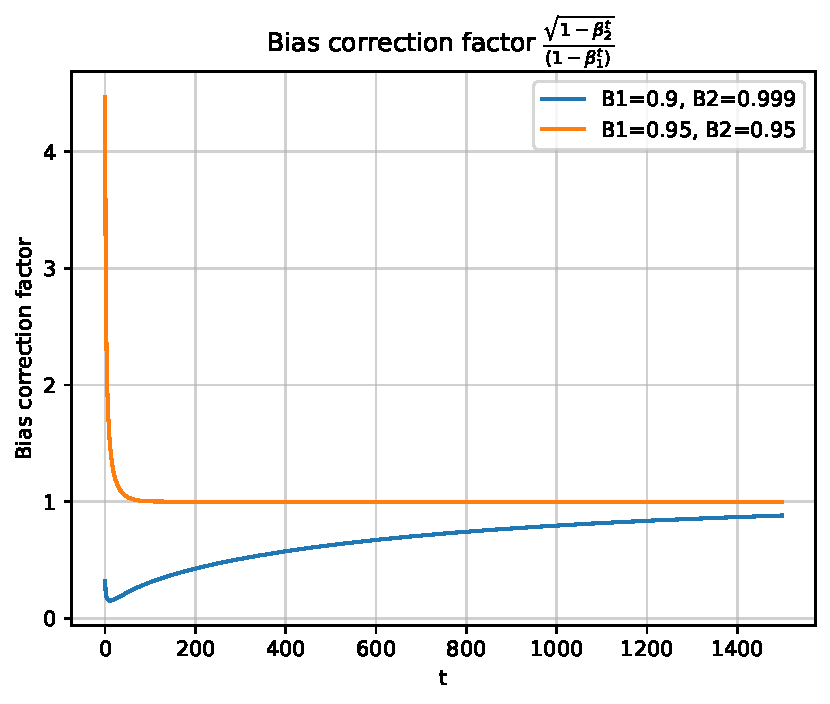
\includegraphics{bias_correction_factor1.pdf}
\\
For the pair $(\beta_1, \beta_2) = (0.9, 0.999)$, the factor resembles a very steady warmup whereas for the pair $(\beta_1, \beta_2) = (0.95, 0.95)$, the factor it merely a large spike which quickly converges to 1\\
\\
Consider the derivative of $\rho$ with respect to $t$:
\begin{align*}
	\frac{d\rho}{dt} &= \cfrac{-\frac{\beta_2^{t}\log\beta_2(1-\beta_1^{t})}{2\sqrt{1-\beta_2^{t}}} + \sqrt{1-\beta_2^{t}} \beta_1^{t}\log\beta_1}{(1-\beta_1^{t})^2} \\
\end{align*}
where $\log$ denotes the natural logarithm. \\
Since $\log\beta_i < 0$ for any $\beta_i \in (0,1)$, we note that $\rho$ has positive $t$-derivative if and only if  
\[
\frac{\beta_2^{t}\log(\beta_2) }{2(1-\beta_2^{t})} < \frac{\beta_1^{t}\log(\beta_1)}{1-\beta_1^{t}}
\]
As we can see, in the case of $(\beta_1, \beta_2) = (0.95, 0.95)$, the derivative is \textit{never} positive. 
\subsection*{Experimental Outline}
We conduct a number of experiment in both a vision and language setting. \\
In the vision setting, we consider:
\begin{itemize}
\item A less overparametrized ResNet implementation on the CIFAR10 dataset (only $\sim 1$M parameters rather than ResNet 18 which has $\sim 11$M)
\item Both a ResNet56\footnotemark{}\footnotetext{Pytorch's ResNet50 was specifically designed for Imagenet's $224\times 224$ images and applies agressive downsampling in the early layers. When applied to CIFAR-100's $32\times 32$ images, important information is then lost and . We therefore make use of a commonly-used specialised ResNet architecture \cite{Idelbayev18a} } and a vision transformer on the CIFAR100 dataset
\item Both a ResNet50 and a vision transformer on the Tiny Imagenet and Imagenet datsets
\end{itemize}
We consider both the pre-training and fine-tuning setting for CIFAR100/TinyImagenet and just the pretraining setting for CIFAR10.\\
\\
In the case of pretraining language models, we restrict our attention to transformer based models. In particular we make use of the \href{https://github.com/Niccolo-Ajroldi/plainLM/tree/main}{following enhanced implementation} of nanoGPT (\cite{Karpathy2022}) including RMSNorm (instead of batch/layer normalization), SwiGLUi\cite{swiGLU} and Rotary Positional Embedding
\\
We note that the exact hyperparemeter configuration used for each experiment is not of integral importance in distinguishing the performance of AdamW with and without bias correction (and indeed zero-initialistion). In each case, we run a sweep to ensure a model of near SOTA performance but this is mainly for vanity and we also consider results across a wide range of hyperparameters to prove the performance similarities are consistent across the space of all hyperparameter configurations. 
\\

\begin{table}[h]
\centering
\caption{\textit{ZI} denotes Zero init, \textit{BC} denotes Bias Correction. Not doing ZI means we initialize $m$ and $v$ at $g_0$ and $g_0^2$ respectively. Default for AdamW is ZI and BC. Performing bias correction is not as important as initialization in Adam. Averaged results over 4 random seeds\\
HPs $\text{lr:}0.008, \beta_1:0.95, \beta_2: 0.95, wd:0.1$}
\vspace{0.5em}
\begin{tabular}{lcccc}
\toprule
& AdamW & AdamW no BC, ZI & AdamW BC, no ZI  &AdamW no BC, no ZI  \\
\midrule
Val ppl & $21.87 \pm 0.11$ & $21.93 \pm 0.04$ & $22.83 \pm 0.15$ & $22.64 \pm 0.13$  \\
\bottomrule
\end{tabular}
\end{table}
It appears that what is far more important than the inclusion of bias correction is rather the initialization of the moments. One would naively assume that initializing the gradients to what they actually are should outperform setting them to zero. However there are minor improvements to initialising at zero 


\chapter{Beyond Adam: Is Muon the future?}
In recent years, there have been a number of papers which attempt to improve upon Adam(W) by leveraging information about the structure of individual layers. \\
Newton's method, which requires explicit computation of the Hessian matrix, is rarely sufficiently efficient, or even tractable, in deep learning. Similarly, Natural Gradient Descent \cite{NGdescent} makes use of the Fischer information matrix \\
A general principle of stochastic optimizers in the age of deep learning is to approximate local information about the curvature of the loss landscape without needing to explicitely compute the full second derivative. Knowledge of local curvature is known to help prevent becoming stuck in bad local minima.   \\
\\
\\
Let $f:\mathcal{X} \times \Theta \to \mathcal{Y}$ with $\Theta \subset \R^{p}$ denote an arbirary deep neural . The textbook definition of most traditional stochastic optimization algorithms involves initialising $\theta_0 \in \Theta$ and then updating with some rule 
\[
\theta_{t+1} = \theta_t - \eta_t s_t
\] 
for a step size $s_t \in \R^{d}$ which typically depends on the current stochastic gradient.  \\
The vast majority of commonly-used first-order optimizers (e.g. SGD, RMSProp, Adadelta AdamW, Lion) ignore the structure of each individual layer of weights of a deep neural network and treat the parameters simply as a long concatenated vector made up of the flattened parameters of each layer. \\
\\
An idea which has regained popularity in recent years is to exploit the individual structure of each layer of the matrix, leveraging this information to compute update directions tailored to each layer. \\ 
The library \href{https://github.com/modula-systems/modula}{Modula} is built precisely on this notion, explicitely constructing a mathematical object called a \textit{module} (not to be confused with the traditional interpretation in commutative algebra). These 
\\
A current SOTA language model is \cite{moonshot}, which uses a  mixture of experts (MoE) transformer model architecture. The model explicitely uses Muon to optimizer linear (non-embedding) layers. Namely
\\
\section{Related Work}
\section{Understanding Muon}
The idea of Muon stemmed from (\todo{cite the modular norm papers from bernstein})
\\
The following exposition builds on the work of \cite{bernstein2024modulardualitydeeplearning}, \cite{bernstein2025deriving}, \cite{jordan2024muon}, \cite{pethick2025trainingdeeplearningmodels} supplemented with some additional pedagogy and proofs.
\todo{give a nice Muon explanation}
\\

\subsection{Metrized Deep Learning}

\subsection{Dualized Gradients and Metrized Deep Learning}
The paper \cite{bernstein2024modulardualitydeeplearning} reviatalizes an old principle in optimization theory. Namely, the insistance on viewing the gradient as a dual vector. \\
Consider a differentiable loss function $L:\Theta \to \R_{\ge_0}$ with respect to the weight space $\Theta \subseteq \R^{d}$. One can consider the first order Taylor approximation of $L$ about arbitrary
\[
 L(
\] 
\subsection{The Newton Schulz Algorithm}
Under the framework of steepest descent under the RMS $\to$ RMS norm, the crucial step size for linear layers is seen as 


\section{Ablations on Simple Problems}
To gain a better understanding of the dynamics of Muon, we study its behavior in simplified settings using both synthetic data and common toy datasets. Our goal is to examine how Muon compares to SGD and AdamW in these controlled environments, and to identify the minimal conditions under which Muon offers practical advantages.
\\
The experiments were all run with the \href{https://github.com/sam-laing/optimizer_playground/tree/main}{following codebase}

\subsection{Linear Regression}
We consider the case of linear regression with a multi-dimensional output. Namely, consider a datasetThis is the simplest setting in which Muon can be applied as the weights for the one-dimensional output case would not admit a matrix structure. 
Here the dynamics of stochastic optimizers are generally well understood. We strive to understand how Muon behaves in this setting and how it differs from SGD and AdamW. We generate a synthetic dataset as follows:
\begin{itemize}
	\item Generate data $Z\in \R^{Nxd}$ with $z_{ij}\sim \mathcal{N}(0,1)$ (corresponding to $N$ datapoints $x_i \in\R^{d}$) and let $X = [1 | Z] \in\R^{d+1} $ (maybe generate better data than just normal) 
	\item Generate a weight matrix $W^* \in \R^{d\times D}$ from a unit Gaussian $\mathcal{N}(0,1)$
	\item Generate noise $\varepsilon\in \R^{N\times D}$ with $\varepsilon _{ij} \sim e \mathcal{N}(0,1)$ for hyperparameter $e\in\R_{>0}$
	\item Let $Y = XW^* + \varepsilon $ and initialise $W\in\R^{d\times D}$
\end{itemize}
The objective (or loss) function is then given by 
\[
	L(W; X,Y) :=  \\ = \|Y - XW\|_F^{2}  \quad  (*)
\] 
where $\|A\|_F := \sum_{i,j \in [m]\times[n]}^{} {|a_{ij}|^2}$ denotes the Frobenius norm of a matrix. \\
The objective function is manifestly convex in $W$. Indeed, we have 
\begin{align*}
L(W) = \|Y - XW\|_F^2 = \|\text{vec(Y - XW)}\|_2^2 = \|\text{vec}(Y) - (\mathbbm{1}_D \otimes X) \text{vec} (W)\|_2^2  
\end{align*}
which is simply a quadratic function of the form $f(x) = \|y - Ax\|_2^2$ with positive-definite Hessian $2A^{T}A$. \\
While such a simple problem admits an analytic solution (indeed $W^* = (X^{T}X)^{-1}X^{T}Y$ provided $X^{T}X$ is invertible), we study the case where the number of datapoints is large   
\\
We experiment with both mini-batch and full gradient methods. \\
The gradient of $(*)$ is given by 
\begin{align*}
	\nabla_W L &= \nabla_W \text{tr}\left((Y - XW)^{T} (Y - XW)\right)\\
		   &= \nabla_W [\text{tr}(Y^TY)  - 2\text{tr}(W^{T}X^{T} Y) + \text{tr}(W^{T}X^{T}XW)]   \\
		   &= 2X^{T}(XW - Y)
\end{align*}
The stochastic gradient for minibatch $(X_t, Y_t)\subset \R^{N\times d} \times \R^{N\times D}$ $t\in\N$, which we denote by $G_t$, is given by 
\[
	G_t = \nabla_{W_t} L(W_t) = 2X_t^{T} (X_tW_t - Y_t)
\]
We consider the singular value decomposition (SVD) $X = U \Sigma V^{T}$ of the feature matrix. 
\\
Then the gradient $G$ (up to a constant) is given by:
 \[
G = X^{T}(XW - Y) = V\Sigma ^{T} U^{T}(U\Sigma V^{T} W - Y) = V^{T}\Sigma^{T}\Sigma \ VW - V\Sigma^{T} U Y
\]
The analytic solution (obtained at $G = 0$ due to convexity) is given by:
\[
	(X^{T}X)^{-1}X^{T}Y = V \Sigma^{-2}V^{T} V \Sigma U^{T}Y = V \Sigma ^{-1} U^{T}Y 
\] 
Since the Muon update dictates considering NewtonSchulz$_n(G_t)$ which is just an approximation of the orthogonalization of $G_t$, we will study the singular value decomposition of $G$ at each time step and study how a variety of factors 
\\
It is well established that the condition number of the feature matrix is a good indicator of the problem's numerical stability and learning difficulty. Therefore we are interested in the interplay between 
\subsection{Logistic Regression}
Similarly to the Linear regression case, we consider multi-class classification with a softmax function. Again, because we are interested in the Muon optimizer, this is the simplest case for which the weights admit a natural matrix structure. 
\\
One can view Logistic regression as a neural network of just one layer so it is certainly worthy of scrutiny.  
\begin{itemize}
\item Generate $X$ and  $W^*$ as in the linear regression case
\item  Let $Z = XW^*$ and  $P = \text{softmax}(Z) + \varepsilon $ for noise $\varepsilon $
\item  Define $Y_{ik} := \begin{cases}
		1, \quad &\text{if $k = \text{argmax}_{\ell \in \{1,\ldots,K\} } P_{i\ell} $}\\
		0, &\text{else}
\end{cases}$\ \ \  for each $i \in\{1,\ldots,N\} $ (or in plain english: each row of $Y$ is a one hot encoded vector in $\R^{K}$)
\item Initialise a random $W\in \R^{(d+1) \times D}$ and compare different optimizer's performance on minimizing loss. 
\end{itemize}
Let $f(X ; W) := \text{softmax}(XW)$
As is standard for classification, we consider the cross-entropy loss:
\[
L(W) = - \cfrac{1}{N} \sum_{i = 1}^{N} \sum_{k=1}^{K} {Y_{ik} \log(P_{ik})} \quad \text{where } P = \text{softmax}(XW)
\]
Let us compute the gradient. We denote $P = \text{softmax}(Z)$  where $Z := XW$. We invoke the chain rule to simplify matters: 
\begin{align*}
\nabla_W L = \nabla_Z L\  . \nabla_W Z = \frac{1}{N} X^{T} (\text{softmax}(XW) - Y)
\end{align*}
\section{SVD structural analysis}
The Muon optimizer makes use of the Newton Schulz algorithm 
\subsection{CIFAR-10 ResNet}
The CIFAR speedrun is a competitive benchmark which aims to achieve a specified test set accuracy in the shortest possible training time (standardized in NVIDIA A100-minutes). Researchers submit their optimizations, which can include network architecture changes, alterations to the training pipeline and test time tricks, and the submission is then benchmarked over a number of random seeds. 
Remarkably, with enhancements using Muon (\todo{cite the right thing}), the record is a mere $2.59$ seconds to achieve 94\% training accuracy. 
\\
We make use of this repository to ablate on some hyperparameter choices for the Muon optimizer. 
\subsubsection*{Comparing Newton Schulz approximation to full Gradient Orthogonalization}


\section{Muon on nanoGPT and plainLM} 
\bibliographystyle{plain}
\bibliography{bibliography}
\end{document} 
